\documentclass[aspectratio=169]{beamer}
\usepackage[T2A]{fontenc}
\usepackage[utf8]{inputenc}
\usepackage[russian]{babel}
\usepackage{graphicx}
\usefonttheme{serif}
\setbeamertemplate{navigation symbols}{}
\setbeamertemplate{footline}{}
\setbeamersize{text margin left=0.55cm,text margin right=0.55cm}
\setbeamercolor{structure}{fg=blue!55!black}
\setbeamerfont{frametitle}{size=\large}

\begin{document}
\begin{frame}{Сохранится ли корреляционный паттерн в объяснении?}
\small
Усиливаем различие групп по Z, сохраняя связь X--Y.
\par\medskip
\centering
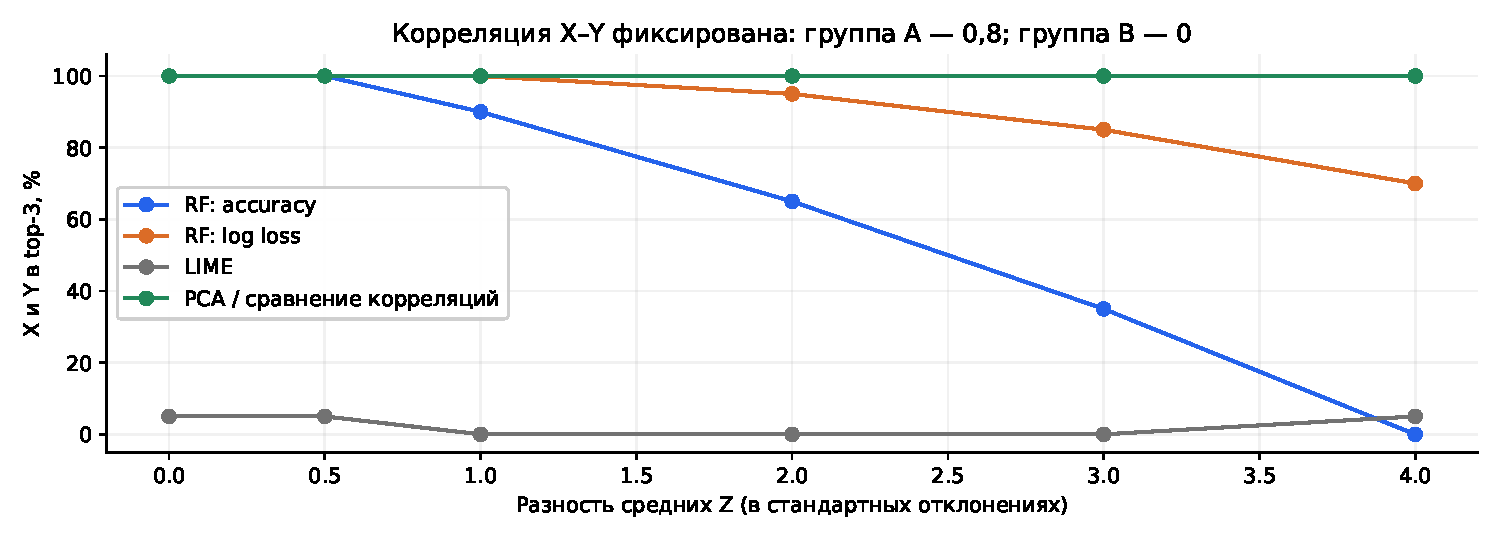
\includegraphics[width=\linewidth,height=4.6cm,keepaspectratio]{../code/figures/slide_figure.pdf}
\par\vspace{0.05cm}
\raggedright
\scriptsize
Top-3 --- три наиболее важных признака; RF --- случайный лес; PCA --- главные компоненты.\par
20 повторов.
\end{frame}
\end{document}
